
\section{TAHOE --- A Cyberthreat Language}\label{sec:tahoe}

Any CIS platform like CYBEX-P potentially handles hundreds of different data formats. Thus, it needs a standard data format and structure to represent threat data. A cyberthreat language (CTL) is a specification of how to format and serialize any kind of threat data. CYBEX-P uses TAHOE instead of other CTLs like STIX\cite{barnum2012standardizing} or MISP\cite{dulaunoy-misp-core-format-13}. TAHOE structures threat data as JSON \cite{bray2014javascript} documents. In this section we introduce TAHOE as a better alternative to other CTLs and directly compare TAHOE with STIX and MISP. The complete TAHOE specification is available on GitHub \cite{sadique2021tahoe}.



\subsection{TAHOE Data Instance}\label{ss:instance}

A piece of TAHOE data is called an \T{instance} and there are $5$ types of TAHOE \T{instances} ---
\begin{enumerate}
    \item \textbf{Raw} A \T{raw} data instance stores unprocessed user data.
    \item \textbf{Attribute} The most basic datatype that holds a single piece of information, like an IP address. Fig. \ref{fig:aef} shows an email address \T{attribute}.
    \item \textbf{Object} Groups several \T{attributes} together, e.g., a file \T{object} may have a filename and a file-size \T{attribute}. Fig. \ref{fig:tof} shows a TAHOE \T{object} with two \T{attributes}.
    \item \textbf{Event} An \T{event} consists of one or more \T{attributes} or \T{objects} along with a \T{timestamp}. \T{Events} structure \T{attributes} or \T{objects} into complete threat data. Fig. \ref{fig:te} shows and email \T{event}.
    \item \textbf{Session} A \T{session} groups arbitrarily related \T{events} (e.g. events when a user visits a website).
\end{enumerate}


\begin{figure}[!ht]
    \footnotesize
    \captionsetup[subfigure]{
        aboveskip=-0.8\baselineskip,
        font={footnotesize,bf},
        justification=justified,
        singlelinecheck=false,
    }
    \begin{minipage}{.29\textwidth}
        \begin{subfigure}{\linewidth}

            \begin{verbatim}
{"itype": "attribute",
"sub_type": "email_addr",
"data": "jdoe@example.com",
"_hash": "5f07..."}
            \end{verbatim}

            \caption{Attribute `from-email-addr'}
            \label{fig:aef}
        \end{subfigure}\\[0.5\baselineskip]
        \begin{subfigure}{\linewidth}

            \begin{verbatim}
{"itype": "attribute",
"sub_type": "name",
"data": "John Doe",
"_hash": "22af..."}
            \end{verbatim}

            \caption{Attribute `from-name'}
            \label{fig:anf}
        \end{subfigure}\\[0.5\baselineskip]
        \begin{subfigure}{\linewidth}

            \begin{verbatim}
{"itype": "attribute",
"sub_type": "email_addr",
"data": "mary@example.com",
"_hash": "b591..."}
            \end{verbatim}

            \caption{Attribute `to-email-addr'.}
            \label{fig:aet}
        \end{subfigure}
    \end{minipage}%
    \hfill
    \begin{minipage}{.29\textwidth}
        \begin{subfigure}{\linewidth}

            \begin{verbatim}
{"itype": "attribute",
"sub_type": "name",
"data": "Mary Smith",
"_hash": "4c90..."}
            \end{verbatim}

            \caption{Attribute `to-name'.}
            \label{fig:ant}
        \end{subfigure}\\[0.5\baselineskip]
        \begin{subfigure}{\linewidth}
            \begin{verbatim}
{"itype": "attribute",
"sub_type": "subject",
"data": "Saying Hello",
"_hash": "50f2..."}
            \end{verbatim}
            \caption{Attribute `email-subject'.}
            \label{fig:asub}
        \end{subfigure}\\[0.5\baselineskip]
        \begin{subfigure}{\linewidth}

            \begin{verbatim}
{"itype": "object",
"sub_type": "from",
"_cref": ["5f07..","22af.."],
"_ref": ["5f07..","22af.."],
"_hash": "d722..."}
            \end{verbatim}

            \caption{Object `from'.}
            \label{fig:tof}
        \end{subfigure}
    \end{minipage}%
    \hfill
    \begin{minipage}{.4\textwidth}
        \begin{subfigure}{\linewidth}

            \begin{verbatim}
{"itype": "object",
"sub_type": "to",
"_cref": ["4c90..","b591.."],
"_ref": ["4c90..","b591.."],
"_hash": "da09..."}
            \end{verbatim}

            \caption{Object `to'.}
            \label{fig:tot}
        \end{subfigure}\\[0.5\baselineskip]
        \begin{subfigure}{\linewidth}

            \begin{verbatim}
{"itype": "event",
"sub_type": "email",
"orgid": "test_org",
"timestamp": 880127706.0
"_cref": ["50f2..","da09..","d722.."],
"_ref": ["4c90..","d722..","5f07..",
    "22af..","da09..","b591..","50f2.."],
"_hash": "f70b..."}
            \end{verbatim}

            \caption{Event `email'.}
            \label{fig:te}
        \end{subfigure}
    \end{minipage}
    \caption{An email event in TAHOE Format. The complete representation of the email consists of $8$ JSON documents. Each document is a node in the TAHOE graph. \texttt{\_hash} is the globally reproducible and unique ID of a document. \texttt{\_cref} stores the edges from objects and events to their children. \texttt{\_ref} stores the edges to both children and grandchildren and so on. The graph is visualized in Fig. \ref{fig:email_tahoe_graph}.}
    \label{fig:email_tahoe}
\end{figure}

\begin{figure}
    \begin{subfigure}{0.45\textwidth}
        \centering
        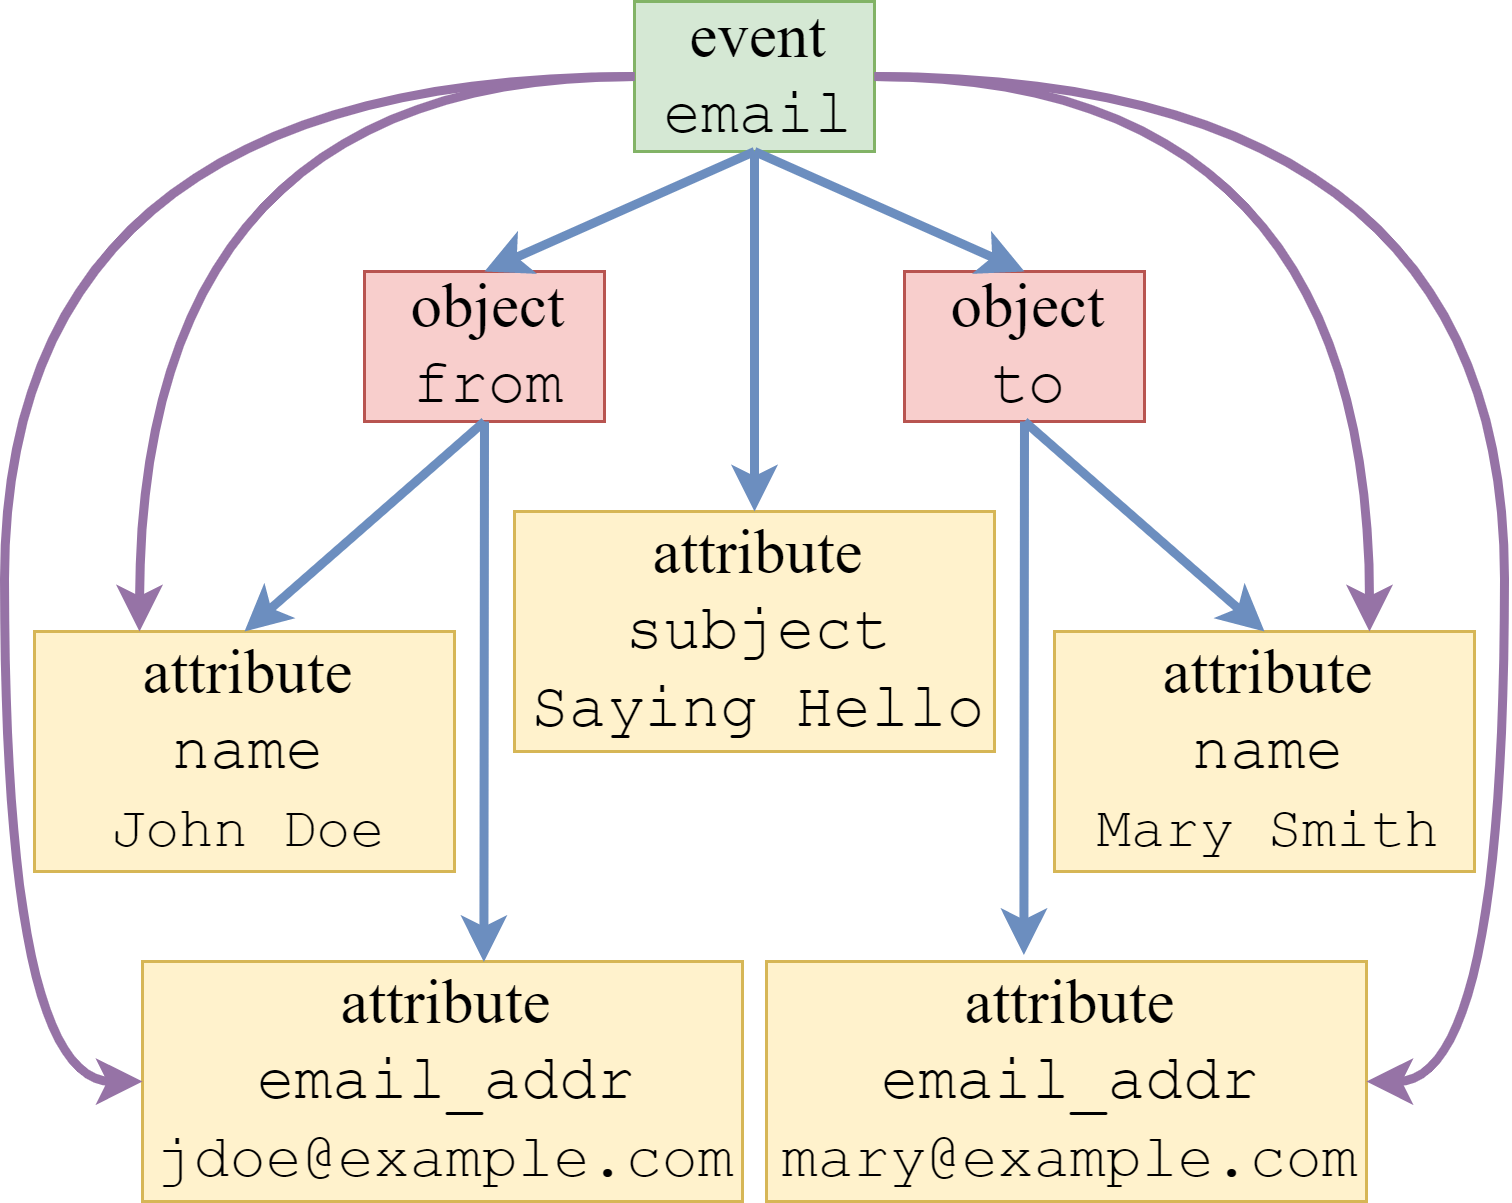
\includegraphics[width=\linewidth]{email_tahoe_graph}
        \caption{The email event as a graph with $8$ nodes and $11$ edges.}
        \label{fig:email_tahoe_graph}
    \end{subfigure}
    \hfill
    \begin{subfigure}{0.23\textwidth}
        \centering
        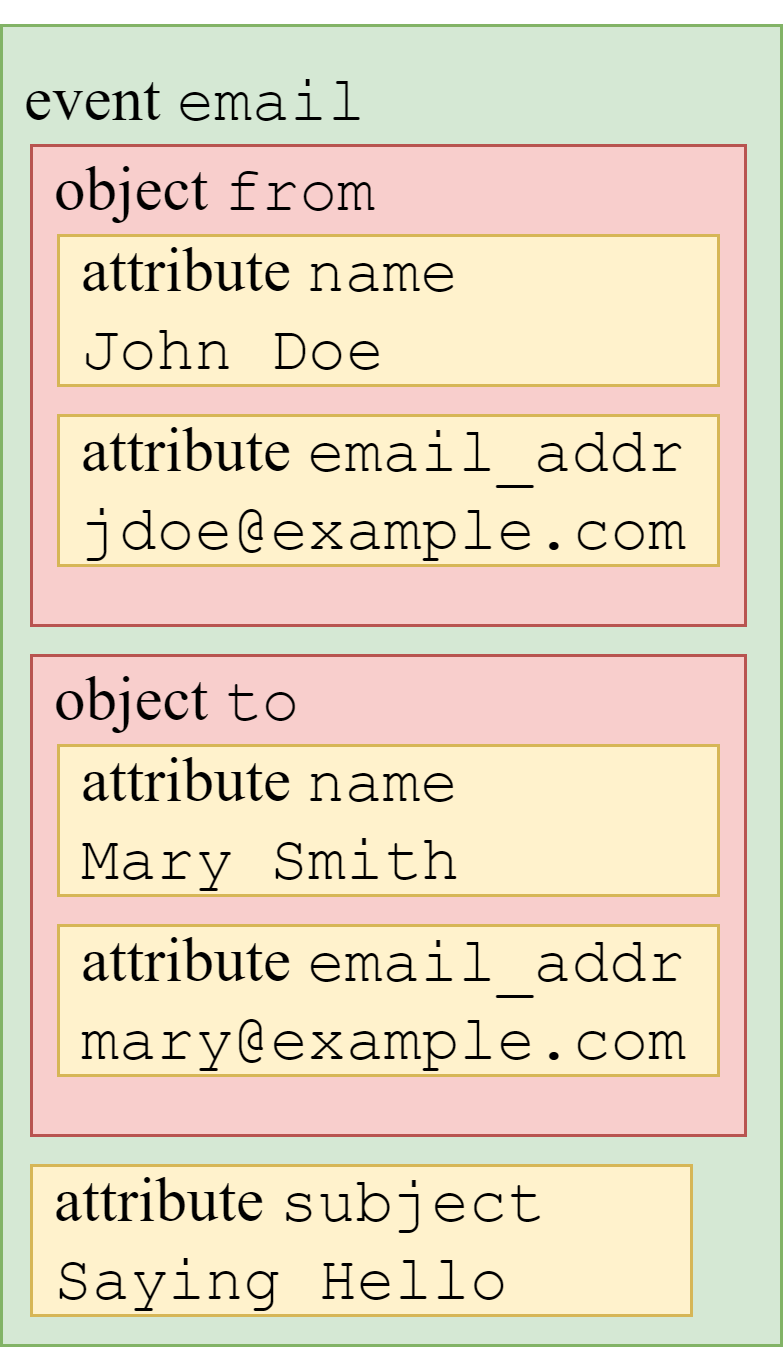
\includegraphics[width=\linewidth]{email_tahoe_nested}
        \caption{The email event as a nested document.}
        \label{fig:email_tahoe_nested}
    \end{subfigure}
    \hfill
    \captionsetup[subfigure]{aboveskip=-0.5\baselineskip}
    \begin{subfigure}{0.26\textwidth}
        \footnotesize

        \begin{verbatim}
"email": {
  "from": [{
     "email_addr": [
        "jdoe@example.com"],
     "name": ["John Doe"]
     }],
  "to": [{
     "email_addr": [
        "mary@example.com"],
     "name": ["Mary Smith"]
     }],
  "subject": [
     "Saying Hello"]
}
        \end{verbatim}

        \caption{The email event as a nested JSON document.}
        \label{fig:email_tahoe_data}
    \end{subfigure}
    \caption{The email event (green) from Fig. \ref{fig:email_tahoe} as a TAHOE graph and a nested document of objects (red) and attributes (yellow).}
    \label{fig:email_tahoe_repr}
\end{figure}



\subsection{Data Structured as Graphs}\label{ss:graph}

TAHOE structures data as graphs, where each TAHOE instance is a graph node.  Fig. \ref{fig:email_tahoe} shows an email structured in TAHOE format. Fig. \ref{fig:email_tahoe_graph} visualizes the email as a TAHOE graph with $8$ nodes and $11$ edges.

As seen from Fig. \ref{fig:email_tahoe}, attributes store actual value or data. Objects and events, on the other hand, do not store any actual data. So, the complete representation of the object in Fig. \ref{fig:tof} must include the attributes in figures \ref{fig:aef} and \ref{fig:anf}. Similarly, the complete representation of the email event in Fig. \ref{fig:te} must also include the other $7$ documents.

As shown in Fig. \ref{fig:email_tahoe} all TAHOE documents have a field called \T{"\_hash"}. The value of this field is derived from the SHA256 hash of the document and serves as a unique identifier for this document. For example, the string `\T{attributesubject"Saying Hello"}' is an unique representation of the subject attribute in Fig. \ref{fig:asub}. We can calculate the SHA256 checksum of this string to be `\T{50f2...}'. This checksum is the unique identifier of the attribute \T{subject="Saying Hello"} in any TAHOE database.

Ojects and events have an array field called \T{"\_cref"}. The \T{"\_cref"} field stores graph edges. For example, the \T{"object-from"} in Fig. \ref{fig:tof} has \T{"\_cref"= ["5f07..","22af.."]}. This indicates, the object is connected to the attributes in Fig. \ref{fig:aef} and in Fig. \ref{fig:anf}. Similarly, the event in Fig. \ref{fig:te} is connected to two objects in Figures \ref{fig:tof} and \ref{fig:tot} and also the attribute in Fig. \ref{fig:asub}. Fig. \ref{fig:email_tahoe_graph} shows these edges as blue arrows.

The array \T{"\_ref"} stores graph edges to all subsequent nodes including children and grandchildren. This field is used for making queries faster and explained in subsection \ref{ss:tahoeVstix}. Both the blue and purple edges from Fig. \ref{fig:email_tahoe_graph} are stored in \T{"\_ref"}. Note, how the event contains complete information about the email just by referring to the other objects and attributes.


% Benefits of this graphical structure are justified in \ref{ss:fcorr}. Also, note that, we draw the edges as arrows because of how edge data is stored in \T{\_ref}. However, in TAHOE database, a graph can be traversed from both end, as explained in \ref{sss:biq}. Objects can also refer other objects if required.

\begin{figure}[!ht]
	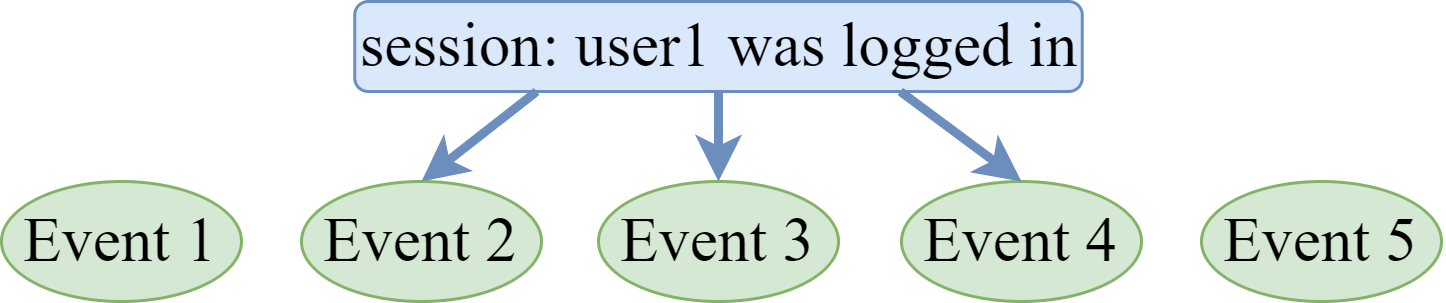
\includegraphics[height=.6in]{session} %height = 10*.06
	\centering
	\caption{Events grouped by arbitrary session parameter.}
	\label{fig:session}
\end{figure}

Finally, A TAHOE session is an arbitrary grouping of related events. This allows us to group events based on any condition the user desires. The session in Fig. \ref{fig:session} groups $3$ events, recorded while $user1$ was logged in.



\paragraph{\textbf{Events Viewed as Nested Documents}}

Although, TAHOE structures events as graphs, they can be viewed as nested documents. Fig. \ref{fig:email_tahoe_nested} shows the email event from Fig. \ref{fig:email_tahoe} as a nested document. Furthermore, Fig. \ref{fig:email_tahoe_data} shows the JSON representation of the nested document. This JSON document is obtained by traversing the graph starting from the event node. The graph edges are stored in the \T{\_cref} arrays. Analysts can choose to view an event as a document or as a graph depending on their need. For all kinds of machine analysis (e.g query), however, the graphical structure of Fig. \ref{fig:email_tahoe_graph} is more suitable.



\subsection{Representing Complex Data -- TAHOE vs. MISP}\label{ss:tahoeVmisp}

\begin{figure}[!ht]
\begin{subfigure}{0.35\textwidth}
        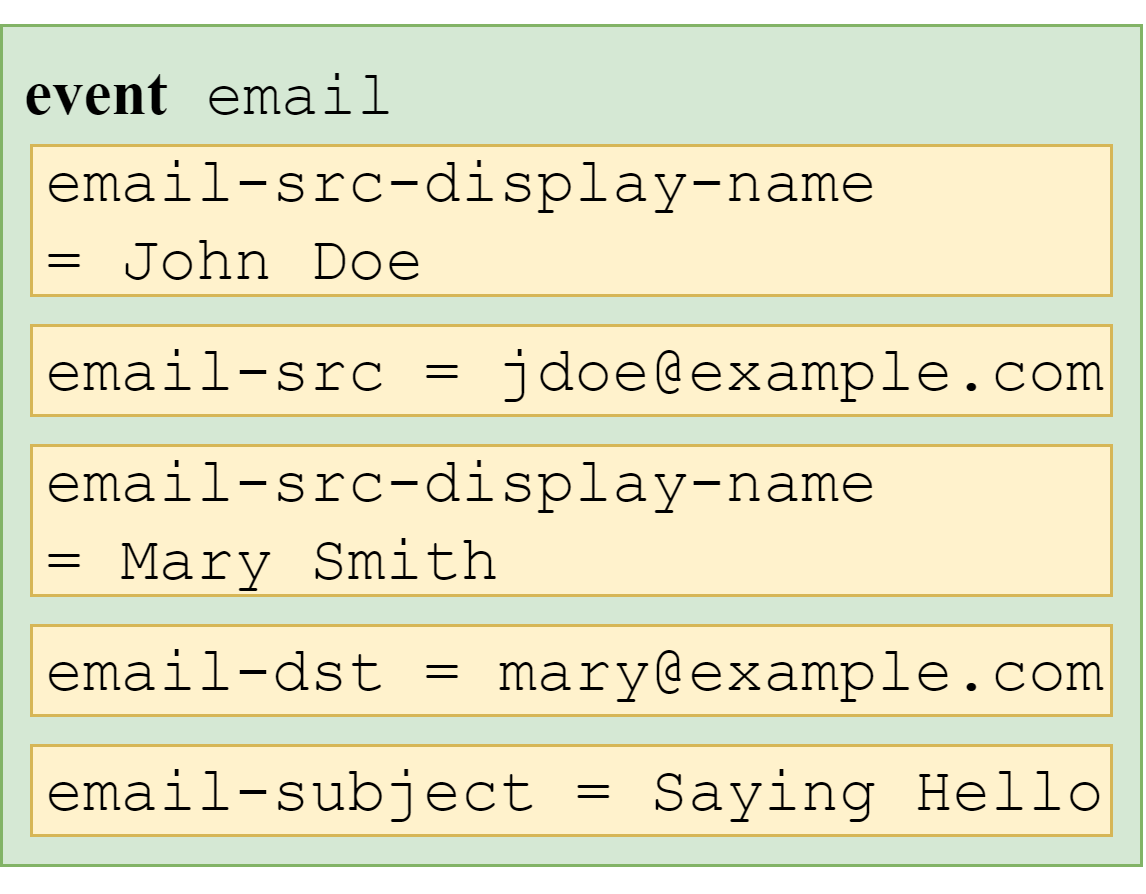
\includegraphics[height=1.6in]{email_misp} %height = 30*.06
    	\centering
    	\caption{The email in Fig. \ref{fig:email_tahoe} as MISP format. MISP struggles to structure complex data and specifies non-intuitive \texttt{attribute} types.}
    	\label{fig:email_misp}
\end{subfigure}
\hfill
\captionsetup[subfigure]{aboveskip=-0.5\baselineskip}
\begin{subfigure}{0.32\textwidth}
    \footnotesize
    \begin{verbatim}
{
"0": {
    "type": "email-addr",
    "value": "jdoe@example.com",
    "display_name": "John Doe"
    },
"1": {
    "type": "email-addr",
    "value": "mary@example.com",
    "display_name": "Mary Smith"
    },
"2": {
    "type": "email-message",
    "from_ref": "0",
    "to_refs": ["1"],
    "date": "1997-11-21T15:55:06Z",
    "subject": "Saying Hello"
    }
}
    \end{verbatim}
    \caption{The email in Fig. \ref{fig:email_tahoe} as STIX format.}
    \label{fig:email_stix}
\end{subfigure}
\hfill
\begin{subfigure}{0.3\textwidth}
    \footnotesize
    \begin{verbatim}
{
"0": {
    "type": "ipv4-addr",
    "value": "1.2.3.4",
    "belongs_to_refs": ["3"]
    },
"1": {
    "type": "ipv4-addr",
    "value": "2.3.4.5"
    },
"2": {
    "type": "network-traffic",
    "src_ref": "0",
    "dst_ref": "1",
    }
"3": {
    "type": "as"
    "number": 42
    }
}
    \end{verbatim}
    \caption{A network packet in STIX format.}
    \label{fig:net_stix}
\end{subfigure}
    \caption{The email event from figures \ref{fig:email_tahoe} and \ref{fig:email_tahoe_repr} in MISP and STIX format and a network packet in STIX format.}
\end{figure}


Traditional CTLs like MISP often struggle to represent complex data. For example, Fig. \ref{fig:email_misp} shows the email event from Fig. \ref{fig:email_tahoe} in MISP \cite{dulaunoy-misp-core-format-13} format.

The key problem is, \T{email-src} and \T{email-dst} are two different attribute-types. So, to fetch all emails to and from \T{jdoe@example.com}, one has to perform $2$ queries -- \T{email-src = jdoe@example.com} and \T{email-dst = jdoe@example.com}. Moreover, MISP represents a lot of information in the attribute-type. So MISP data structure includes cumbersome attribute-types like \T{passenger-name-record-locator-number} or non-intuitive attribute-types like \T{filename|md5, filename|sha224, filename|sha256} etc.

Firstly, TAHOE can store arbitrarily complex data because TAHOE objects can be infinitely nested and can refer other objects. As seen if Fig. \ref{fig:email_tahoe}, TAHOE has simple attribute types like, \T{email\_addr} or \T{subject}. Secondly, a TAHOE event is connected to all of its attributes via the \T{\_ref} array. So, to fetch all emails to and from \T{jdoe@example.com}, TAHOE requires only $1$ query -- \T{email\_addr = jdoe@example.com}.



\subsection{Indexing \& Scalability -- TAHOE vs. STIX}\label{ss:tahoeVstix}

Earlier in section \ref{sec:rw}, we claimed that, ``While STIX is perfect for mutual data sharing, it is unscalable for any kind of data analysis.'' This subsection provides a detailed explanation in support of our claim. Since, both STIX and TAHOE use JSON documents we will have to store them in a NoSQL database. For this discussion, we consider the most popular NoSQL database - MongoDB \cite{banker2011mongodb}.

Consider, the STIX document in Fig. \ref{fig:email_stix}. It has $3$ keys - \T{"0"}, \T{"1"}, \T{"2"}. Here, \T{"0"} and \T{"1} are JSON objects with $3$ keys each whereas \T{"2"} is a JSON object with $5$ keys. Assume, we want to \textit{fetch all emails from jdoe@example.com}. The MongoDB syntax for that query is, \T{find(\{"0.value":"jdoe@example.com"\})}.\footnote{The actual query is \texttt{find(\{"0.type":"email-addr","2.type":"email-message","0.value":"jdoe@example.com"\})}. We have shortened the queries in the example for clarity.} This query will get all JSON documents in the database which have \T{"0.value"="jdoe@example.com"}. Similarly, if we want to \textit{fetch all emails with subject="Saying Hello"} the query is \T{find(\{"2.subject": "Saying Hello"\})}.

Now, these queries will take forever in a decent sized database unless we index the keys \T{"0.value"} and \T{"2.subject"}. Similarly, in Fig. \ref{fig:net_stix}, to efficiently lookup all the network traffic events of \T{"type"="as"}, we must index the \T{"3.type"} key. Eventually, for these two event types, we must index a total of $16$ keys -- \T{"0.type", "0.value", "0.display\_name", "1.type", "1.value", "1.display\_name", "2.type", "2.from\_ref", "2.to\_refs", "2.date", "2.subject", "0.belongs\_to\_refs", "2.src\_ref", "2.dst\_ref", "3.type", "3.number"}. Indexing in this manner creates $3$ problems for us:

\begin{enumerate}
    \item Not all documents have all the keys. For instance, the network traffic event in Fig. \ref{fig:net_stix} does not have the \T{"2.subject"} key. So, the indexing will be inefficient.
    \item MongoDB only allows $64$ keys to be indexed in a database collection. As discussed earlier, we have $16$ keys only for two types of events. As we encounter, more event types with arbitrary structures, we will have hundreds of keys that need indexing. Indexing so many keys is not feasible.
    \item Some, fields have large values. For example, RFC2322 states that the email subject has no length restrictions. Which means the \T{"2.subject"} field in Fig. \ref{fig:email_stix} can be larger than $1024$ bytes. However, MongoDB cannot index a field larger than $1024$ bytes. So, large fields in a STIX document can never be indexed.
\end{enumerate}

Going back to our earlier discussion, queries like \T{find(\{"0.value": "jdoe@example.com"\})} will be too slow in a database if the fields are not indexed. That is why we claim that STIX is unscalable for data analytics.

TAHOE incorporates a novel solution to these challenges. Consider the query \textit{fetch all emails with subject="Saying Hello"}. This is a two-step process in TAHOE --

\begin{enumerate}
    \item We create the string `\T{attributesubject"Saying Hello"}'. This string is an unique representation of this subject attribute. We then calculate the SHA256 checksum of this string to be `\T{50f2...}'. This checksum is the unique identifier of the attribute \T{subject="Saying Hello"} in any TAHOE database.
    \item In the second step, we perform the following MongoDB query - \T{find(\{"\_ref": "50f2..."\})}. \footnote{The actual query is \texttt{find(\{"itype":"event", "sub\_type":"email", "\_ref": "50f2..."\})}.} \footnote{We have made a TAHOE backend library that interfaces with MongoDB to automate the whole query process. So, users will not actually have to calculate the checksums and then query the MongoDB. The library is available at https://github.com/cybex-p/tahoe}
\end{enumerate}

These two steps will return all the emails which have \T{subject="Saying Hello"}. In terms of TAHOE graph, we are essentially querying all events which are connected the TAHOE attribute \T{subject="Saying Hello"}.

Now, in TAHOE, we only query one key - \T{"\_ref"}; so, we only index this one key. Therefore, we will never pass the $64$ keys limit of MongoDB. Also, all events have the \T{"\_ref"} field, so the indexing will be efficient. Finally, each element in the \T{"\_ref"} array is a SHA256 checksum, which means each of them are $256$ bits long. So, we will not violate the $1024$ bytes limit on indexed fields. Thus TAHOE takes care of all the $3$ problems mentioned earlier for STIX.

\begin{figure}[!ht]
    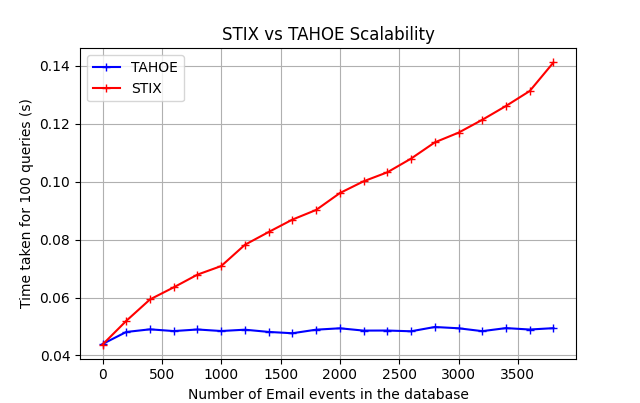
\includegraphics[height=2.5in]{stixVtahoe} %height = 31*0.06
    \centering
    \caption{Scalability of STIX vs TAHOE. The x-axis is the total number of email events in the database. The y-axis is the total time taken for $1000$ queries in the databases. The query for the STIX database is \texttt{find(\{"0.value": "jdoe@example.com"\})}. The query for the TAHOE database is \texttt{find(\{"\_ref": "50f2..."\})}.}
    \label{fig:stixVtahoe}
\end{figure}

Fig. \ref{fig:stixVtahoe} compares the scalability STIX 2.0 and TAHOE. The graph compares the time take for the \T{find(\{"0.value": "jdoe@example.com"\})} query for the STIX database with the \T{find(\{"\_ref": "50f2..."\})} query for the TAHOE database. The x-axis is the total number of email events in the database. The y-axis is the total time taken for $100$ queries in the databases. The plot clearly shows that the time-required grows linearly with the database size for STIX. This is because the key \T{"0.value"} is not indexed and every query becomes a linear search in the database. The time-required for the TAHOE database, however, stays constant as the number of emails grows in the database. This is because the key \T{"\_ref"} is indexed in the database. And since indexed keys are stored as hash-tables in the RAM, every lookup takes roughly the same time despite the size of the database.



\subsection{Intrinsic Correlation of Graphical Data}\label{ss:fcorr}


\begin{figure}[!ht]
\begin{subfigure}{0.32\textwidth}
	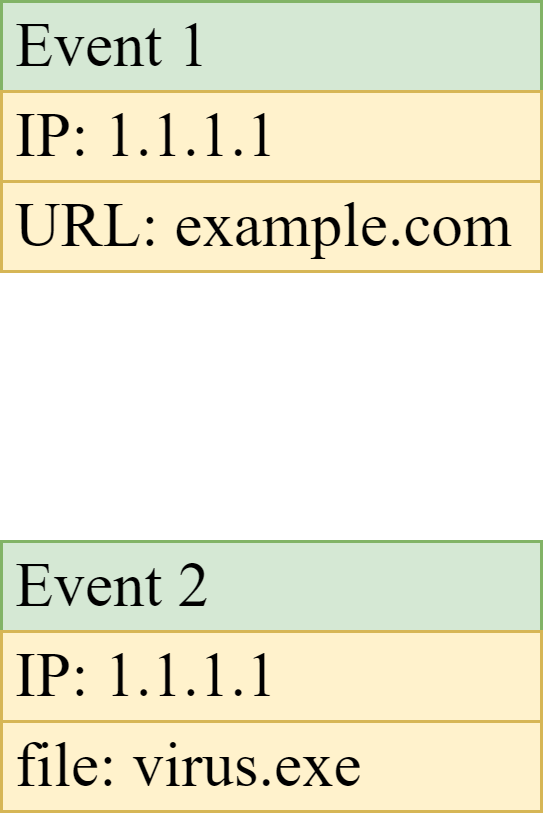
\includegraphics[height=1.6in]{event_doc} % height = 5*.15 (5 lines in notepad++)
	\centering
	\caption{Two events as separate documents.}
	\label{fig:event_doc}
\end{subfigure}
\hfill
\begin{subfigure}{0.32\textwidth}
	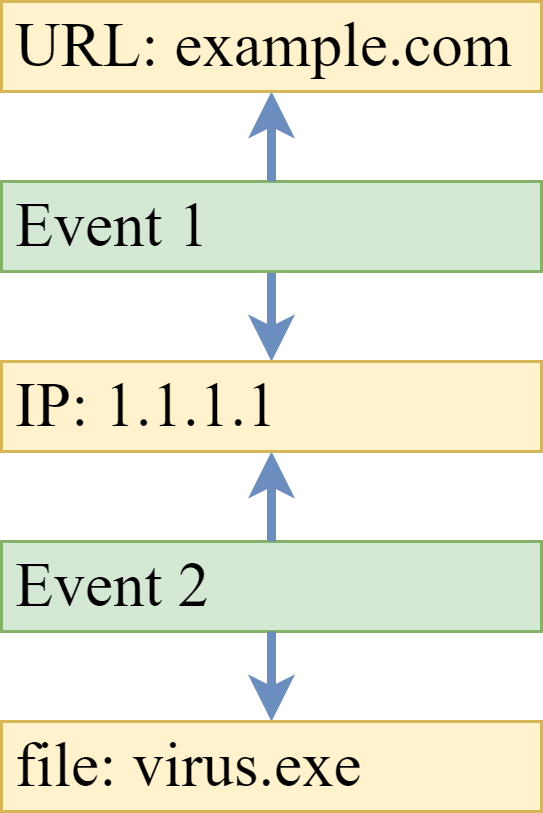
\includegraphics[height=1.6in]{event_tahoe} % height = 5*.15 (5 lines in notepad++)
	\centering
	\caption{Two events as TAHOE graph.}
	\label{fig:event_tahoe}
\end{subfigure}
\hfill
\begin{subfigure}{0.32\textwidth}
	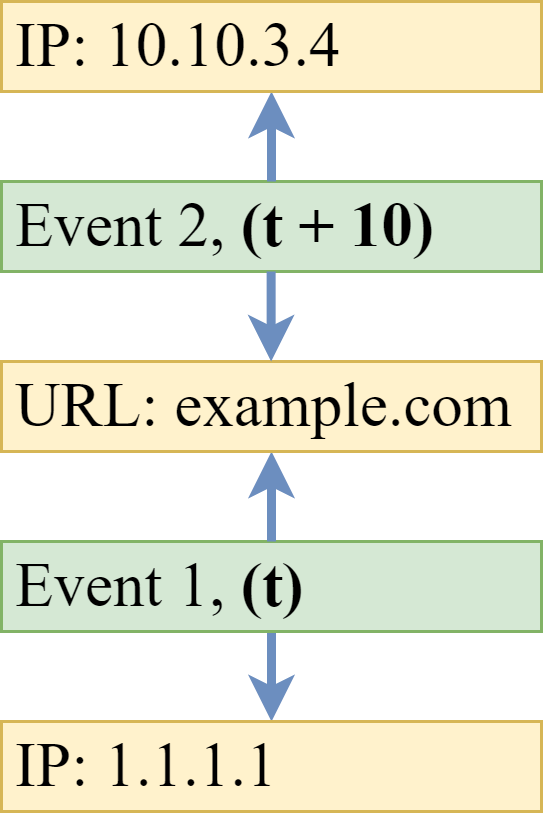
\includegraphics[height=1.6in]{event_tahoe_time} % height = 5*.15 (5 lines in notepad++)
	\centering
	\caption{A time-varying attribute.}
	\label{fig:event_tahoe_time}
\end{subfigure}
    \caption{Fig. \ref{fig:event_tahoe} shows how TAHOE intrinsically correlates the two separate events from Fig. \ref{fig:event_doc} based on their common attribute. Fig. \ref{fig:event_tahoe_time} shows an example TAHOE graph for a time-varying attribute.}
    \label{fig:tahoe_corr}
\end{figure}

Traditional CTLs, store threat data as separate documents like shown in Fig. \ref{fig:event_doc}. These data are difficult to analyze because the events lack any direct correlation with own attributes. TAHOE, on the other hand, represents data as graphs like in Fig. \ref{fig:event_tahoe}. Here, two separate events are automatically connected by their common \T{attribute} (\T{1.1.1.1}) in TAHOE. Such `intrinsic correlation' is a powerful feature of TAHOE, because if someone looks up \T{example.com} she will immediately see that \T{virus.exe} is related to it. This is a major strength of our investigation tool (subsubsection \ref{par:neo4j}). Moreover, we leverage this feature to formulate a novel malicious event detection mechanism in section \ref{sec:pagerank}.

Furthermore, TAHOE can correlate time-varying attributes. As shown in Fig. \ref{fig:event_tahoe_time}, lets assume the Tahoe database records two events - Event 1 at time $\mathbf{t}$ and Event 2 at time $\mathbf{t+10}$. Also assume, During event 1, at time $\mathbf{t}$, the domain  \T{example.com} resolves to \T{1.1.1.1} and during event 2, at time $\mathbf{t+10}$, the domain \T{example.com} resolves to \T{10.10.3.4}. Now, the TAHOE database will connect both the IP addresses to the domain in a graph like that shown in Fig. \ref{fig:event_tahoe_time}.

Please note that, both IP addresses are associated with \T{example.com} after Event 2 is recorded. Also note that, the IPs are not directly connected to \T{example.com}, rather connected via their respective events. For example, \T{1.1.1.1} is connected to \T{example.com} via Event 1 (time $\mathbf{t}$) and \T{10.10.3.4} is connected to \T{example.com} via Event 2 (time $\mathbf{t+10}$).

So, if someone queries \T{example.com}, they will be able to see the complete graph in Fig. \ref{fig:event_tahoe_time} including the timestamps. From, the graph any person or machine can deduce that \T{example.com} was associated with \T{1.1.1.1} at time $\mathbf{t}$ and was associated with \T{10.10.3.4} at time $\mathbf{t+10}$. Thus, the time aspect of the relationship is preserved.

Moreover, users can specify time ranges when querying the TAHOE database to filter out one of these events. For example, if any user or machine queries events related to \T{example.com} between $\mathbf{t+5}$ and $\mathbf{t+15}$, they will only see Event 2 in the graph.



\subsection{Features of TAHOE}


\subsubsection{\textbf{Data Normalization}} TAHOE normalizes different formats of same type of data. Consider two firewalls from two different vendors. Their log data will be formatted differently despite having same type of data. TAHOE normalizes such differences by converting them into the same structure.


\subsubsection{\textbf{Data De-duplication}}\label{sss:dup}

TAHOE prohibits duplicate data. For example, there can only be one instance of the IP $1.1.1.1$ in a TAHOE database. This saves CYBEX-P a lot of storage by not storing the same IP in different \T{events}. TAHOE achieves this de-duplication of data by creating a globally reproducible hash of the data.


\subsubsection{\textbf{Database Independence}}

%graph database \cite{angles2008survey}

Although TAHOE is a graph based CTL we did not use a graph database as a container for TAHOE. In other words, all the information, including the edge data, of a TAHOE graph is stored in the JSON documents of the TAHOE \T{instances}, as shown in Fig. \ref{fig:email_tahoe}.

Furthermore, as described in \ref{ss:tdql} we have developed a universal threat data query language (TDQL) to communicate with any TAHOE storage. These two contributions make TAHOE a database-independent CTL.


\subsubsection{\textbf{Optimized for Indexing}}\label{sss:idx}

Subsection \ref{ss:tahoeVstix} discusses how TAHOE is optimized for indexing in databases and compares the query performance of a STIX database with that of a TAHOE database. The ability to query related data is a novel feature of TAHOE and enables CYBEX-P to perform advanced analytics on TAHOE data.


\subsubsection{\textbf{Globally Unique \& Reproducible Data for Conflict-free Sharing}}

\begin{figure}[ht]
	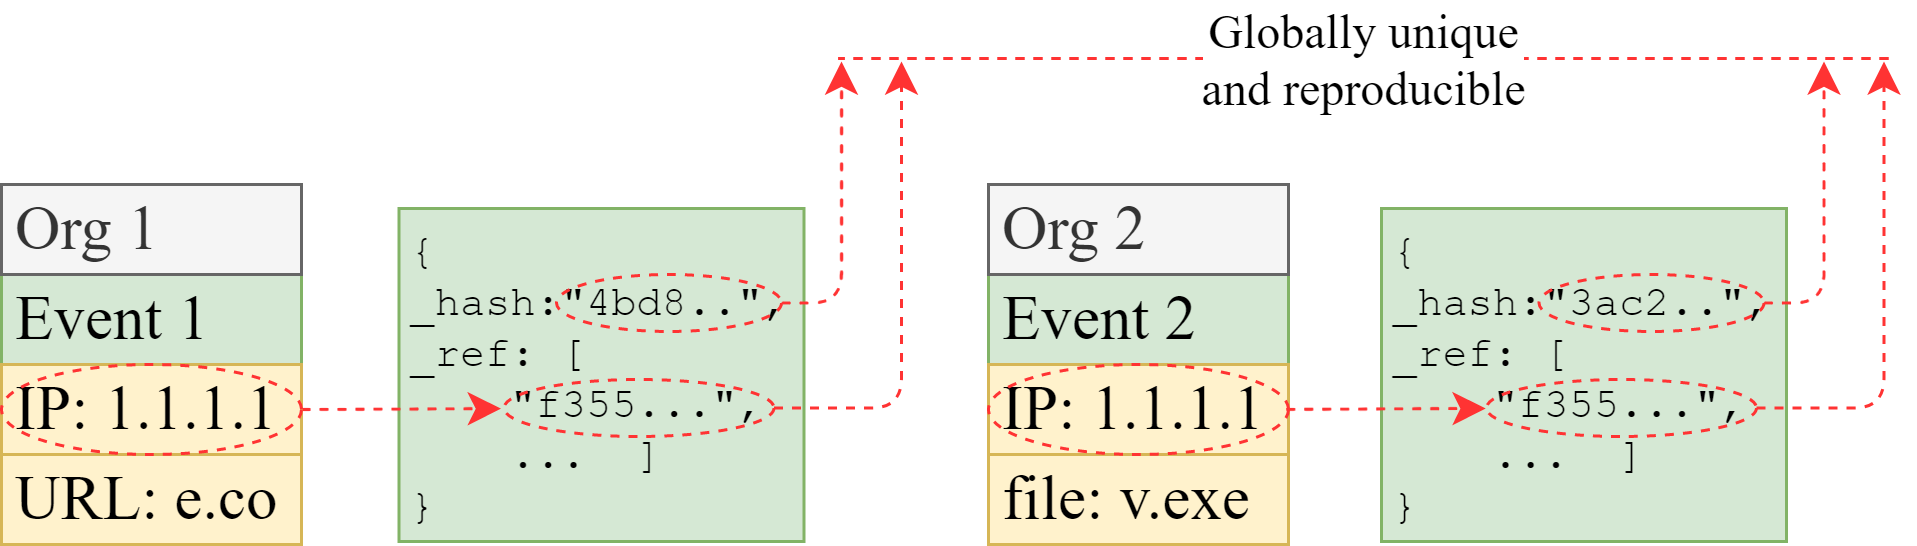
\includegraphics[height=1.2in]{reproducible_id_edge}
	\centering
	\caption{TAHOE id and edges are globally unique and reproducible, making them collision free.}
	\label{fig:repedge}
\end{figure}

TAHOE data are globally unique and reproducible. As shown, in Fig. \ref{fig:repedge}, the IP \T{1.1.1.1} has the same unique id (its hash) in two different organizations. Consider, \T{Org 1} shares \T{Event 1} with \T{Org 2}. If \T{Org 2} had a different id for \T{1.1.1.1} it would have to update the \T{\_ref} array of \T{Event 1}. But, as hashes are reproducible yet unique, this is not required. Note that, event hashes include a timestamp (not shown in figure). Hence, two separate events will have different hashes even if they have same attributes.


\subsubsection{\textbf{Bidirectional Edges for Versatile Queries}}\label{sss:biq}

TAHOE edges are bidirectional. As seen in Fig. \ref{fig:repedge}, edge data is stored in the \T{event} only. This is because, an IP like $8.8.8.8$ (public DNS) can potentially get connected to millions of \T{events}. If we store the hash of all these \T{events} in the IP \T{attribute}, it would result in an unbounded growth of its edge array. So, we store the edge info in the \T{events}. However, it takes only one pass over the database, to get all \T{events} that have a particular hash in their edge array. So, the edges are bidirectional for all intents and purposes.



\subsection{Threat Data Query Language (TDQL)}\label{ss:tdql}

TAHOE aims to standardize the structuring of threat data in terms of \T{attributes, objects, events} and \T{sessions}. This would allow users to query threat data using those terms. An example query could be \T{fetch all events which include the attribute 1.1.1.1}. At present this is not possible because \T{event} or \T{attribute} are not standardized terms for any existing database. For example, if a person queries an SQL database for \T{events} it would not know what to return, because \T{event} is not a standard term for SQL.

% SQL \cite{hursch1988sql}

To that end, we have developed a universal threat data query language (TDQL) for TAHOE. TDQL acts as a layer between a database and a user.  Additionally, TDQL is tailor made for threat data and addresses their nuances. While SQL depends on the structure of database tables, TDQL speaks in terms of \T{attributes, objects, events} etc. So, irrespective of the data storage or delivery protocol, a user can always fetch any threat data from any database.

Additionally, having a dedicated TDQL makes TAHOE, database-independent. However, detailed documentation of TDQL is beyond the scope of this research work.





























\iffalse
\subsubsection{\textbf{Attributes in a Malicious Context}}

While a malicious \T{event} (e.g. a spam email) stays malicious for eternity, the same is not true for \T{attributes}. For example, a website can be hacked and used to distribute malware for a week; after which it is restored by the website admin. Here, the website \T{URL attribute} is malicious for a week and becomes benign afterwards.

Similarly, not all \T{attributes} of a malicious \T{event} are malicious. For example, if X receives a spam email from Y, only Y is a malicious \T{attribute} not X. X is the victim and a benign \T{attribute} in this \T{event}.

For these reasons, TAHOE never classifies an \T{attribute} (e.g. an IP) as malicious. Rather TAHOE maintains a special edge, called a \T{\_mal\_ref} between an \T{event} and an \T{attribute}. For example, if an IP \T{1.1.1.1} is seen in a malicious context in a firewall log \T{event}, the IP is connected by a \T{\_mal\_ref} with the log \T{event}. As a result, TAHOE can count the number of times a particular \T{attribute} has been seen in a malicious context vs in a benign context.
\fi

%In summary, CYBEX-P uses TAHOE which stores data as graphs. TAHOE leverages existing graph algorithms and basic graph operations to generate deep insights into seemingly unrelated cyberthreat data. To the best of our knowledge such correlations have not been studied in the cybersecurity industry making CYBEX-P and TAHOE a novel endeavor.





















\iffalse
\subsection{Data Query by Graph Manipulation}\label{ss:query}

As discussed earlier, traditional CTLs do not support versatile queries. In this subsection, we discuss how simple graph manipulations result in queries in TAHOE.

Then the \T{events} connected to those timestamps automatically become related. This is how CYBEX-P performs a query in a particular datetime range.

\begin{figure}[ht]
	\includegraphics[width=3in]{tahoe2}
	\centering
	\caption{TAHOE \T{events} with time vertices (a) separate (b) collapsed}
	\label{fig:tahoe2}
\end{figure}

The example in Fig. \ref{fig:tahoe2} shows how collapsing all vertices from $5$pm to $7$pm connects the corresponding \T{events}. Now, we can query all \T{events} connected to this collapsed vertex to get the \T{events} ($2, 3, 4$) between $5$pm and $7$pm.

\begin{figure}[ht!]
	\includegraphics[width=1.8in]{tahoe5}
	\centering
	\caption{Sequential graph of \T{events} sorted by their timestamp}
	\label{fig:tahoe5}
\end{figure}

The next example in Fig. \ref{fig:tahoe5} shows how we can get a sequential graph of \T{events} sorted by their timestamps. First, we create directed edges from lower timestamps to greater timestamps. Then we collapse each \T{event} with its own timestamp. Thus using two basic graph operations we obtain the \T{events} in order of when they were generated.

\begin{figure}[ht]
	\includegraphics[height=1.05in]{tahoe4} %height = 15*.07
	\centering
	\caption{Events grouped by arbitrary session parameter}
	\label{fig:tahoe4}
\end{figure}

Yet another method by which \T{events} are correlated in TAHOE are sessions. A session is an arbitrary grouping of related \T{events}. This allows us to group together \T{events} based on any condition we desire. Figure \ref{fig:tahoe4} shows grouping $3$ events generated while $user1$ was logged into the system.

\begin{figure}[ht!]
	\includegraphics[width=2in]{tahoe3}
	\centering
	\caption{Combining two filters in a query}
	\label{fig:tahoe3}
\end{figure}

Finally, we can combine two or more filters to further narrow down the scope as  in Fig. \ref{fig:tahoe3}. Here, we query the database for \T{events} connected to both $4$pm$-7$pm and $1.1.1.1$ and get \T{events} $2$ and $3$ in return.

\fi

















\iffalse





\subsection{Data Structured as Graphs}


\begin{figure}[!ht]
	\includegraphics[height=.9in]{0xa1} % height = 6*0.15 (6 lines in notepad++)
	\centering
	\caption{A TAHOE \T{ip Attribute}; \T{\_hash} also serves as id.}
	\label{fig:0xa1}
\end{figure}

Fig. \ref{fig:0xa1} shows a TAHOE \T{ip attribute}. Each TAHOE \T{instance} (\T{attribute}, \T{object}, \T{event} etc.) has a \textbf{\T{\_hash}} property calculated as the the SHA256 \cite{dworkin2015sha} digest of all other fields and serves as the unique \textbf{id} for that instance. Here, for example, it is the SHA256 of the $<$\T{itype,sub\_type,data}$>$ string (Fig. \ref{fig:0xa1} lists an example value for \T{\_hash}).

\begin{figure}[!ht]
	\includegraphics[height=2.70in]{0xb1} % height = 18*0.15
	\centering
	\caption{A TAHOE \T{file Object} as a graph.}
	\label{fig:0xb1}
\end{figure}

Fig. \ref{fig:0xb1} shows a TAHOE \T{file object} with $2$ \T{attributes}. As seen, the \T{file} object does not include the actual \T{filename} and \T{filesize} (bytes), rather references them in the \textbf{\T{\_ref}} field. So, its complete representation includes these \T{attributes} in the outermost array.

The \T{\_ref} field essentially makes the data a graph with $3$ nodes (\T{0xA2.., 0xA3.., 0xB2..}) and $2$ edges (\T{0xA2.. $\gets$ 0xB2.., 0xA3.. $\gets$ 0xB2..}).

\begin{figure}[!ht]
	\includegraphics[height=2.55in]{0xe1} % height = 17*0.15
	\centering
	\caption{A TAHOE \T{file\_download Event} (truncated)\\as a graph of \T{objects} and \T{attributs}.}
	\label{fig:0xe1}
\end{figure}

Fig. \ref{fig:0xe1} shows a truncated TAHOE \T{file\_download event} with $2$ \T{objects}. This \T{event} refers $2$ \T{objects} -- \T{0xB1..} (Fig. \ref{fig:0xb1}) and \T{0xB2..}. So, both the \T{objects} and their \T{attributes} must be included in the array (truncated in figure). Events can also refer \T{attributes} directly. \T{\_malicious\_score} and \T{\_mal\_ref} are explained in \ref{sec:pagerank}.








\fi















\iffalse

On the other end of the spectrum, we have TAXII \cite{connolly2014trusted}, which structures data as STIX. TAXII by default stores data in a NoSQL database (MongoDB), to support arbitrary data structures. However, there are hundreds of threat data types (IP, email address, URL etc.), while only $64$ types can be indexed in MongoDB. Querying un-indexed data takes more than hours in a reasonably sized TAXII server, making it practically unfeasible.

TAHOE  tackles these challenges by employing a set of novel techniques. Firstly, . , as shown in Fig. \ref{fig:nestedgeneral}.

 Secondly, a TAHOE \T{event} refers all subsequent \T{nodes} up to the leaf, not only the next node. This is depicted in Fig. \ref{fig:tahoeref1}, by the edges -- \T{event} $\rightarrow$ \T{object n} and \T{event} $\rightarrow$ \T{attribute}. As a result, any TAHOE \T{event} is always $1$ database query away from it's \T{attributes} no matter the level of nesting.


\begin{figure}[!ht]
    \begin{subfigure}{0.48\textwidth}
	\includegraphics[height=1.8in]{emaildoc} %height = 12*.15
	\centering
	\caption{A TAHOE \T{email event} as a nested JSON document.}
	\label{fig:emaildoc}
    \end{subfigure}
    \begin{subfigure}{0.48\textwidth}
    	\includegraphics[height=1.48in]{emailgraph} %height = 24*.06
    	\centering
    	\caption{A TAHOE \T{email event} as a graph.}
    	\label{fig:emailgraph}
    \end{subfigure}
\end{figure}

Finally, going back to the example of Fig. \ref{fig:misp}, we can structure an \T{email} in TAHOE as Figures \ref{fig:emaildoc} and \ref{fig:emailgraph}. Note that both the source and destination email addresses are stored in TAHOE \T{email attributes}, not two different \T{attributes} like MISP. So, fetching all emails to and from \T{doe@example.com} will take only one query. Moreover, as all the \T{events} connected to \T{doe@example.com} are zero hop away, the query is fast.



Finally, TAHOE databases do not have to index all \T{attribute} types, rather just $2$ fields -- (1) the \T{\_hash} field to lookup an \T{attribute} and the \T{\_ref} to lookup related \T{events}. This is explained in detail in \ref{sss:idx}.


\fi